\documentclass[a4j]{jarticle}
\usepackage{amsmath}
\usepackage{ascmac}
\usepackage{amssymb}
\usepackage{enumerate}
\usepackage{multicol}
\usepackage{framed}
\usepackage{fancyhdr}
\usepackage{latexsym}
\usepackage{indent}
\usepackage{cases}
\usepackage[dvips]{graphicx}
\allowdisplaybreaks
\pagestyle{fancy}
\lhead{}
\chead{}
\rhead{東京大学前期$1973$年$1$番}
\begin{document}
%分数関係


\def\tfrac#1#2{{\textstyle\frac{#1}{#2}}} %数式中で文中表示の分数を使う時


%Σ関係

\def\dsum#1#2{{\displaystyle\sum_{#1}^{#2}}} %文中で数式表示のΣを使う時


%ベクトル関係


\def\vector#1{\overrightarrow{#1}}  %ベクトルを表現したいとき(aベクトルを表現するときは\ver
\def\norm#1{|\overrightarrow{#1}|} %ベクトルの絶対値
\def\vtwo#1#2{ \left(%
      \begin{array}{c}%
      #1 \\%
      #2 \\%
      \end{array}%
      \right) }                        %2次元ベクトル成分表示
      
      \def\vthree#1#2#3{ \left(
      \begin{array}{c}
      #1 \\
      #2 \\
      #3 \\
      \end{array}
      \right) }                        %3次元ベクトル成分表示



%数列関係


\def\an#1{\verb|{|$#1$\verb|}|}


%極限関係

\def\limit#1#2{\stackrel{#1 \to #2}{\longrightarrow}}   %等式変形からの極限
\def\dlim#1#2{{\displaystyle \lim_{#1\to#2}}} %文中で数式表示の極限を使う



%積分関係

\def\dint#1#2{{\displaystyle \int_{#1}^{#2}}} %文中で数式表示の積分を使う時

\def\ne{\nearrow}
\def\se{\searrow}
\def\nw{\nwarrow}
\def\ne{\nearrow}


%便利なやつ

\def\case#1#2{%
 \[\left\{%
 \begin{array}{l}%
 #1 \\%
 #2%
 \end{array}%
 \right.\] }                           %場合分け
 
\def\1{$\cos\theta=c$,$\sin\theta=s$とおく.}  %cs表示を与える前書きシータ
\def\2{$\cos t=c$,$\sin t=s$とおく.}     %cs表示を与える前書きt
\def\3{$\cos x=c$,$\sin x=s$とおく.}                %cs表示を与える前書きx

\def\fig#1#2#3 {%
\begin{wrapfigure}[#1]{r}{#2 zw}%
\vspace*{-1zh}%
\input{#3}%
\end{wrapfigure} }           %絵の挿入


\def\a{\alpha}   %ギリシャ文字
\def\b{\beta}
\def\g{\gamma}

%問題番号のためのマクロ

\newcounter{nombre} %必須
\renewcommand{\thenombre}{\arabic{nombre}} %任意
\setcounter{nombre}{2} %任意
\newcounter{nombresub}[nombre] %親子関係を定義
\renewcommand{\thenombresub}{\arabic{nombresub}} %任意
\setcounter{nombresub}{0} %任意
\newcommand{\prob}[1][]{\refstepcounter{nombre}#1[問題 \thenombre]}
\newcommand{\probsub}[1][]{\refstepcounter{nombresub}#1(\thenombresub)}


%1-1みたいなカウンタ(todaiとtodaia)
\newcounter{todai}
\setcounter{todai}{0}
\newcounter{todaisub}[todai] 
\setcounter{todaisub}{0} 
\newcommand{\todai}[1][]{\refstepcounter{todai}#1 \thetodai-\thetodaisub}
\newcommand{\todaib}[1][]{\refstepcounter{todai}#1\refstepcounter{todaisub}#1 {\bf [問題 \thetodai.\thetodaisub]}}
\newcommand{\todaia}[1][]{\refstepcounter{todaisub}#1 {\bf [問題 \thetodai.\thetodaisub]}}


     \begin{oframed}
     $S$を中心$O$,半径$a$の球面とし,$N$を$S$上の一点とする.点$O$において線分$ON$と$\pi/3$の角度で交わる
     ひとつの平面の上で,点$P$が点$O$を中心とする等速円運動をしている.その角速度は毎秒$\pi/12$であり,また
     $|OP|=4a$である.点$N$から点$P$を観測するとき,$P$は見え始めてから何秒間見え続けるか.また$P$が見え始めた時点
     から見えなくなる時点までの,$|NP|$の最大値および最小値を求めよ.ただし,球面$S$は不透明であるものとする.
     \end{oframed}

\setlength{\columnseprule}{0.4pt}
\begin{multicols}{2}
{\bf[解]} \1 ただし$0\le\theta<2\pi$とする.
$P$が$xy$平面上の円$x^2+y^2=16a^2$上を動くよう,$N(a/2,0,\sqrt{3}a/2)$とする.
すると$P(4ac,4as)$と置ける.$N$での$S$の接平面$T$は
     \[T:\frac{a}{2}x+\frac{\sqrt{3}a}{2}z=a^2\]
であり,これと$xy$平面との交線は$x=2a$となり,下図のようになる.
\vspace{-3zh} 
     \begin{center}
     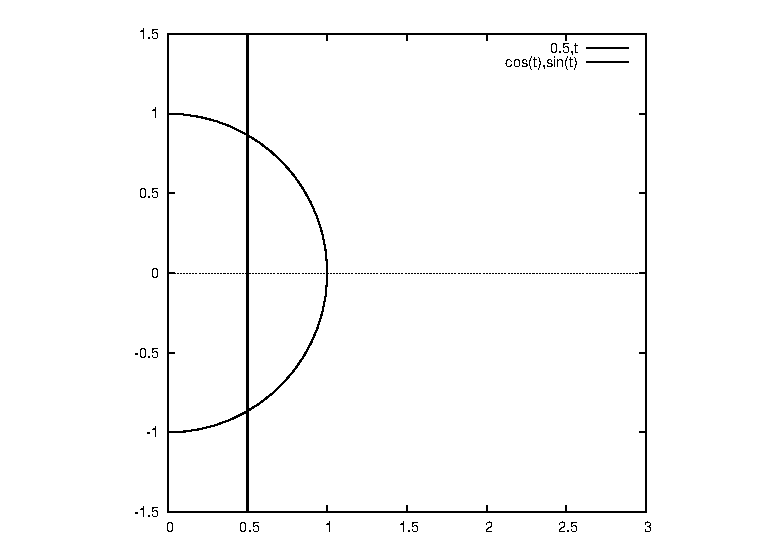
\includegraphics[scale=0.5]{ut-73-1.eps}
     \end{center}
\vspace{2zh}     
$P$が見えるのは$2a\le x$の領域である.これは$-\pi/3\le\theta\le\pi/3$の領域であるから,見え続ける時間$t$として
     \[\frac{\pi}{12}t=\frac{2\pi}{3} \Longleftrightarrow t=8\]
である.$\cdots$(答)

次に,$f(\theta)=|NP|^2$とおくと,
     \begin{align*}
     f(\theta)&=\left(4ac-\frac{a}{2}\right)^2+(4as)^2+\left(\frac{\sqrt{3}a}{2}\right)^2 \\
     &=a^2\left[16c^2-4c+\frac{1}{4}+16s^2+\frac{3}{4}\right] \\
     &=a^2\left[-4c+17\right]
     \end{align*}
である.この$-\pi/3\le\theta\le\pi/3$での最大小を求めればよく,$|NP|\ge0$ゆえ,
     \begin{align*}
          &\begin{cases}
          \max f(\theta)=f\left(\pm\dfrac{\pi}{3}\right)=15a^2 \\
          \min f(\theta)=f(0)=13a^2
          \end{cases} \\
     \therefore \ 
          &\begin{cases}
          \max |NP|=\sqrt{15}a \\
          \min |NP|=\sqrt{13}a
          \end{cases} 
     \end{align*}
である.$\cdots$(答)
\newpage
\end{multicols}
\end{document}